
\documentclass[11pt]{article}
\usepackage[a4paper,margin=1in]{geometry}
\usepackage{graphicx}
\usepackage{hyperref}
\usepackage{siunitx}
\title{System Health Monitor: KPI Trending, Anomaly Detection, and Reliability Analytics}
\author{Ahmad Ali}
\date{\today}
\begin{document}
\maketitle

\begin{abstract}
This report documents a lightweight system health monitoring application for a power-station balance-of-plant system. Using mock, public data, it computes availability-style KPIs, detects anomalies in multivariate sensor streams, and estimates failure behavior using a simple Weibull fit, exposed through a minimal Flask dashboard. The intent is to demonstrate system engineering workflows for trending, troubleshooting, and maintenance prioritization.
\end{abstract}

\section{Introduction}
System engineers maintain awareness of system condition via KPIs, adverse trend detection, and reliability insights. Industry initiatives have emphasized streamlining health reports toward high-value KPIs while retaining a focus on equipment reliability (e.g., AP-913-style processes).

\section{Methods}
\subsection{KPIs}
Availability is approximated as the fraction of time flow exceeds a threshold; demand failures are counted from sustained low-flow excursions; open work orders are summarized from event logs.

\subsection{Anomaly Detection}
An Isolation Forest identifies multivariate outliers across flow, differential pressure, temperature, and vibration features, marking timestamps for investigation.

\subsection{Reliability}
Inter-failure intervals are fit to a Weibull distribution using a log-linear plotting-position method to estimate shape $\beta$ and scale $\eta$ for remaining-life intuition.

\section{Results}
Figure~\ref{fig:last24} illustrates the last-24h composite trend of key variables. Figure~\ref{fig:anom} flags outliers in flow for quick triage.
\begin{figure}[h]
\centering
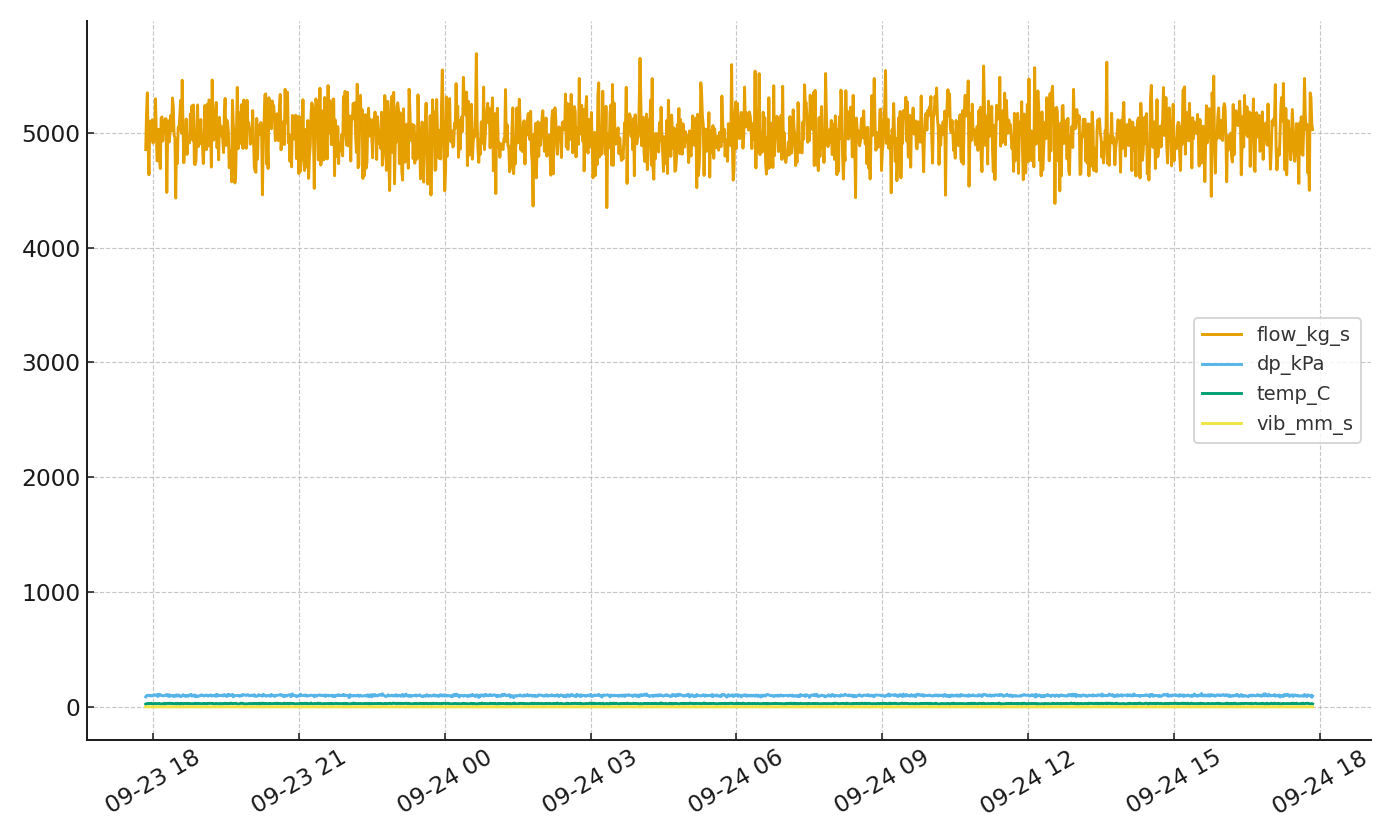
\includegraphics[width=0.95\linewidth]{outputs_last24.png}
\caption{Last-24h trend (mock data).}
\label{fig:last24}
\end{figure}

\begin{figure}[h]
\centering
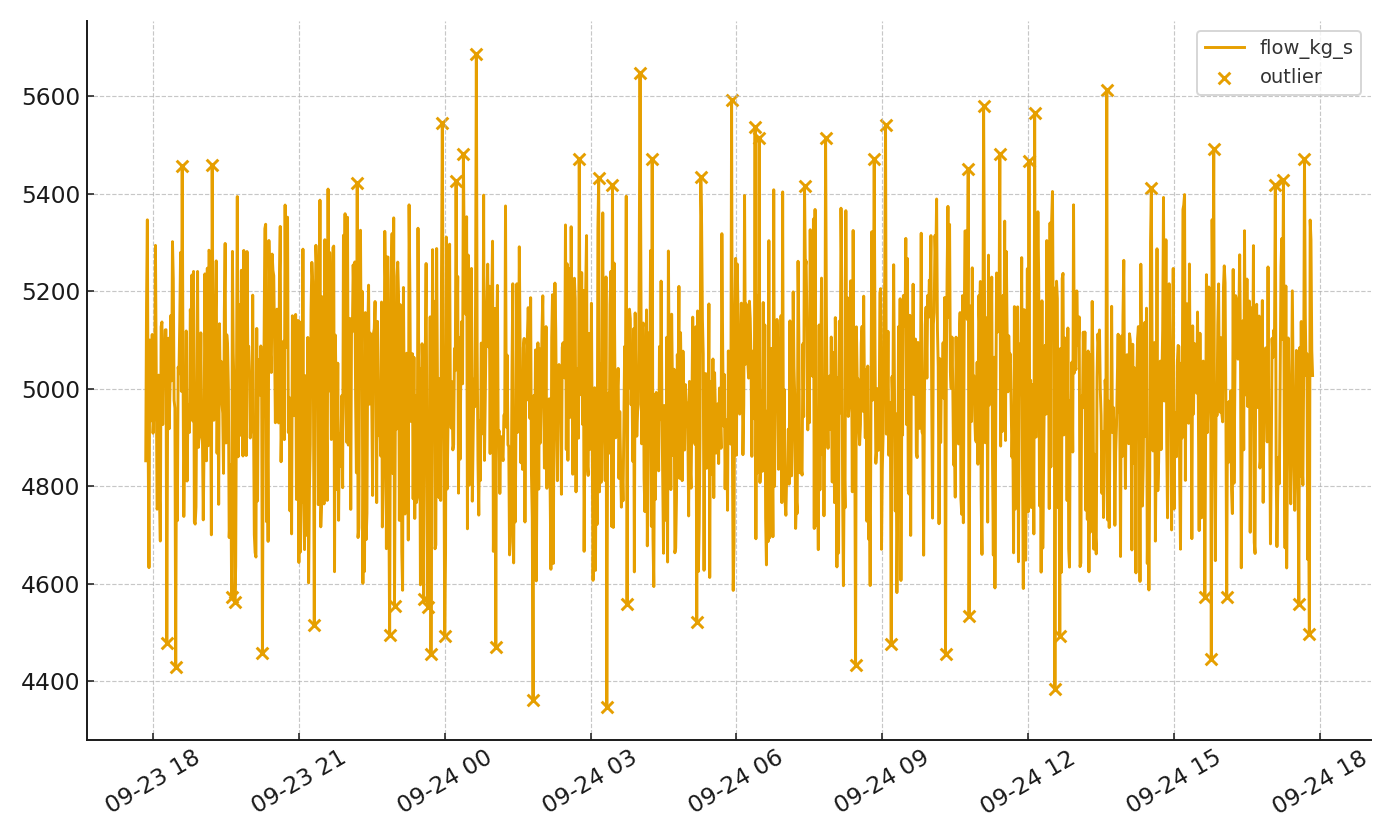
\includegraphics[width=0.95\linewidth]{outputs_anomalies.png}
\caption{Outlier marks on flow (mock).}
\label{fig:anom}
\end{figure}

\section{Discussion}
The app demonstrates a pragmatic backbone for a system health program: concise KPIs, anomaly surfacing, and reliability estimators feeding work prioritization. Integrations to plant historians (e.g., PI) and CMMS (e.g., Maximo) would follow site governance and cybersecurity requirements.

\section{Conclusion}
This example supports system-health storytelling that is clear for leadership and actionable for engineers, aligning with industry moves to streamline reporting while preserving reliability focus.

\appendix
\section{How to Run}
Create a virtual environment, install requirements, generate mock data, and start the Flask server. See repository README.

\section{References (Public Sources)}
\begin{enumerate}
\item NEI EB 16-34: \emph{Streamline Program Health Reporting}. \url{https://www.nei.org/resources/delivering-the-nuclear-promise/eb-16-34-streamline-program-health-reporting}
\item NRC Guidance noting linkage to INPO AP-913: \url{https://www.nrc.gov/docs/ML1204/ML12041A221.pdf}
\item AP-913 overview examples (INIS/EDF experience): \url{https://inis.iaea.org/records/g7byd-nm174}
\end{enumerate}
\end{document}
